\documentclass[10pt,a4paper]{article}
\usepackage{amsmath}
\usepackage{amssymb}
\usepackage{graphicx}
\usepackage{color}
\usepackage{fancyhdr}
\usepackage{fancyvrb}
\usepackage[margin=3.5cm]{geometry}
\usepackage{framed}
\usepackage{enumerate}
\usepackage{textcomp}
\def\ket#1{\left|#1\right\rangle}
\def\bra#1{\left\langle#1\right|}
\def\braket#1{\left\langle#1\right\rangle}

\definecolor{linkcol}{rgb}{0.0, 0.0, 0.5}
\usepackage[colorlinks=true,urlcolor=linkcol,citecolor=black,linkcolor=linkcol]{hyperref}

\setcounter{section}{-1}
\renewcommand\thesection{\arabic{section}}
\renewcommand\thesubsection{\thesection.\arabic{subsection}}

\fancyhf{}
\lhead{\tiny Y.~D.~Chong (2018)}
\rhead{\scriptsize MH2801: Complex Methods for the Sciences}
\lfoot{}
\rfoot{\thepage}
\pagestyle{fancy}

\makeatletter
\def\PY@reset{\let\PY@it=\relax \let\PY@bf=\relax%
    \let\PY@ul=\relax \let\PY@tc=\relax%
    \let\PY@bc=\relax \let\PY@ff=\relax}
\def\PY@tok#1{\csname PY@tok@#1\endcsname}
\def\PY@toks#1+{\ifx\relax#1\empty\else%
    \PY@tok{#1}\expandafter\PY@toks\fi}
\def\PY@do#1{\PY@bc{\PY@tc{\PY@ul
\def\PYZdl{\char`\$}
\def\PYZhy{\char`\-}
\def\PYZsq{\char`\'}
\def\PYZdq{\char`\"}
\def\PYZti{\char`\~}

\begin{document}
    
\section{Mathematical Functions}\label{mathematical-functions}

This is a course on complex methods in the physical sciences. Before
dealing with complex numbers, however, let us undertake a brief review
of real mathematical functions and their properties.

\subsection{Real functions}\label{real-functions}

A mathematical function, denoted $f$, takes an \textbf{input} $x$
(which is also called an \textbf{argument}), and returns an
\textbf{output} $f(x)$. For now, we consider the case where both $x$
and $f(x)$ are real numbers. The set of possible inputs is called the
\textbf{domain} of the function, and the set of possible outputs is
called the \textbf{range}.

A well-defined function must have an unambiguous output: for any $x$
in the domain, $f(x)$ must be a specific number in the range. In other
words, functions must be either one-to-one (injective) mappings, or
many-to-one mappings. They can't be one-to-many or many-to-many. This is
illustrated by the following graphs:

\begin{figure}[h]
  \centering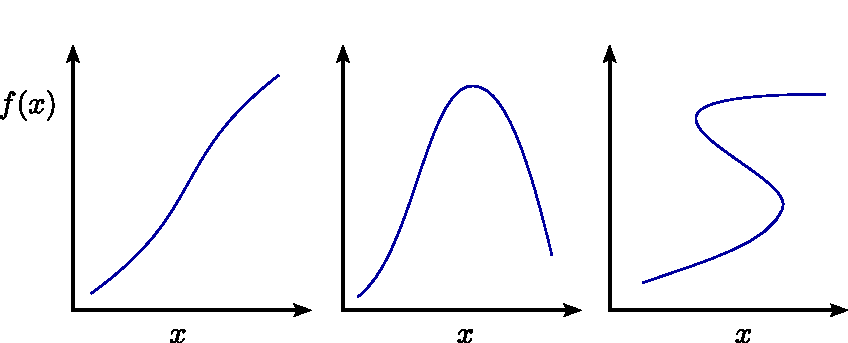
\includegraphics[width=0.7\textwidth]{mathfunctions}
\end{figure}

Simple examples of mathematical functions are those based on elementary
algebra operations:
\begin{align*}
  f(x) = x + 2 \,\;\;\qquad\qquad \text{(a one-to-one function)} \\
  f(x) = x^2 + 2x + 4 \qquad \text{(a many-to-one function)}
\end{align*}

\subsection{The exponential function}

The exponential, conventionally denoted by ``$\exp$'', is an
especially important function. You've probably come across it before,
but let's recall the motivation behind it. We begin by thinking about
what it means to take a number $x$ to the power of $y$:
\begin{equation}
f(x) = x^y.
\end{equation}
For values of $y$ in the natural numbers
$\mathbb{N} \equiv \{1,2,3,\dots\}$, the power operation simply means
multiplying $x$ by itself $y$ times. For example,
$x^4 = x \cdot x \cdot x \cdot x$. But what about non natural number
powers, like $x^{-1}$ or $x^{1/2}$ or $x^{3.14}$?

To help answer this question, we introduce the exponential function,
defined as the following limiting infinite series:
\begin{equation}
\exp(x) \equiv 1 + \sum_{n=1}^\infty\frac{x^n}{n!}, \qquad x \in \mathbb{R}.
\end{equation}
Note that the infinite series in this definition uses natural number
powers only. The domain of this function is the entire set of real
numbers, $\mathbb{R}$, and its range is the set of positive numbers,
$\mathbb{R}^+$.

Here is a graph of the exponential function: 

\begin{figure}[h]
  \centering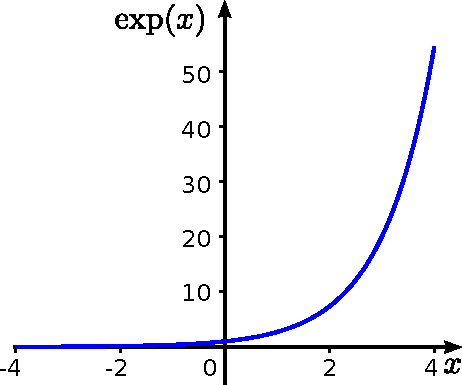
\includegraphics[width=0.4\textwidth]{exponential}
\end{figure}

A noteworthy feature of the exponential is that the value of $exp(x)$
increases extremely quickly with $x$. Going in the other direction,
the value becomes small extremely quickly as we decrease $x$.

Another interesting property of the exponential is that
\begin{equation}
\exp(x+y) = \exp(x)\,\exp(y) \quad \forall x, y \in \mathbb{R}.
\end{equation}
(Try proving this as an exercise.)

As a corollary,
\begin{equation}
\exp(-x) = 1/\exp(x).
\end{equation}

\subsection{The logarithm function}
\label{the-logarithm-function}

Because the exponential is a one-to-one function, its inverse is also a
well-defined function. We call this the \textbf{natural logarithm}:
\begin{equation}
\ln(x) \equiv y \;\; \mathrm{such}\;\mathrm{that}\;\;\exp(y) = x.
\end{equation}
Henceforth, unless otherwise noted, we will simply use the term
``logarithm'' to refer to the natural logarithm. The domain of the
logarithm is $y \in \mathbb{R}^+$, and its range is $\mathbb{R}$.  Its
graph is shown below:

\begin{figure}[h]
  \centering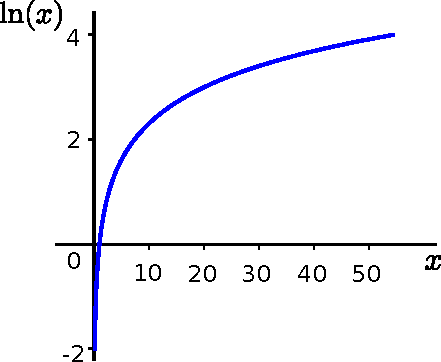
\includegraphics[width=0.4\textwidth]{logarithm}
\end{figure}
\noindent
Observe that for $x>0$, $\ln(x)$ increases very slowly with $x$. This
is the opposite of the exponential function's behavior, where
$\exp(x)$ increases very quickly with $x$.

Using the fact that $\exp(x+y) = \exp(x)\exp(y)$, one can prove that
the logarithm satisfies the property
\begin{equation}
\ln(xy) = \ln(x) + \ln(y).
\end{equation}

\subsection{Non-natural powers}

Having defined the exponential and logarithm functions, we have the
tools needed to address the issue raised earlier, i.e.~how to formulate
the concept of a non-natural power. First, observe that the natural
power operation interacts with the exponential and logarithm functions
in the following manner:
\begin{align}
  \ln(x^y) &= y \ln(x)\qquad\quad&\mathrm{for}&\;\;y \in \mathbb{N} \\
  \Rightarrow\quad\quad x^y &= \exp[y \ln(x)] \quad &\mathrm{for}&\;\;y \in \mathbb{N}.
\end{align}
Now, we generalize the above equation so that it holds for any positive
$x$ and real $y$, not just $y \in \mathbb{N}$. In other words, we
treat this as our \emph{definition} of the power operation for
non-natural powers:
\begin{equation}
x^y \equiv \exp[y \ln(x)] \qquad\; \mathrm{for}\; x \in \mathbb{R}^+, \;y \notin \mathbb{N}.
\end{equation}
By this definition, the power operation always gives a positive
result.  You can also check that, for $y \in \mathbb{N}$, the formula
is consistent with the results based on using the standard definition
of ``multiply $x$ by itself $y$ times''.

This generalization of the power operation leads to several important
consequences:
\begin{itemize}
\item Raising a positive number to the zeroth power gives
  unity: $\displaystyle x^0 = 1.$

\item
  Negative powers are reciprocals:
$\displaystyle x^{-y} = \exp[-y\ln(x)] = \exp[-\ln(x^y)] = \frac{1}{x^y}.$

\item The exponential function can itself can be written as a power:
$\displaystyle\exp(y) = e^y$, where $e \equiv \exp(1) = 2.718281828459\dots$

\item Non-integer powers are only defined for non-negative $x$, since
  the logarithm does not accept negative inputs.
\end{itemize}

\subsection{Trigonometric functions}
\label{trigonometric-functions}

The fundamental trignonometric functions $\sin(\theta)$,
$\cos(\theta)$, and $\tan(\theta)$ can be defined in terms of the
geometric ratios of the sides of right-angled triangles, as shown here:

\begin{figure}[h]
  \centering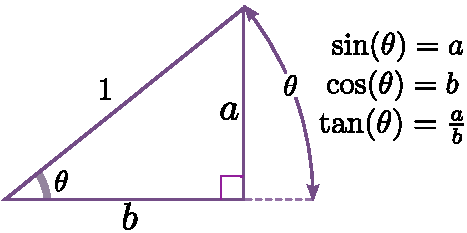
\includegraphics[width=0.37\textwidth]{trigonometry}
\end{figure}

In this basic definition, the domain is $\theta \in [0, \,\pi/2)$,
where the angle $\theta$ is given in radians. We can generalize the
definitions to allow for negative values of $a$ and/or $b$, using
the following scheme:

\begin{figure}[h]
  \centering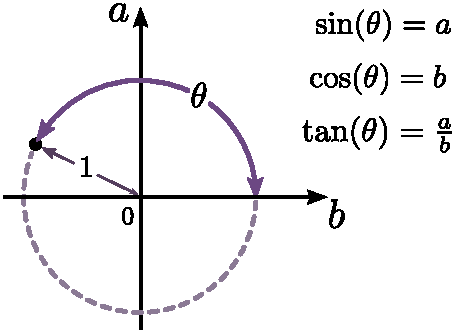
\includegraphics[width=0.37\textwidth]{trigonometry2}
\end{figure}

With this, the angle $\theta$ lies within a larger domain: $\theta \in
[0,\,2\pi)$. We can further generalize the trigonometric functions by
extending the domain to all real numbers: $\theta \in
\mathbb{R}$. This is done by treating all values of $\theta$ modulo
$2\pi$ as equivalent, i.e.  $f(\theta + 2\pi) = f(\theta)$. With this
generalization, the trigonometric functions become many-to-one
functions.

From the
\href{http://en.wikipedia.org/wiki/Pythagoras_theorem}{Pythagorean
theorem} (which can be proved in
\href{http://www.faculty.umb.edu/gary_zabel/Courses/Phil\%20281b/Philosophy\%20of\%20Magic/Arcana/Neoplatonism/Pythagoras/index.shtml.html}{many,
many ways}),
\begin{equation}
\big[\sin(\theta)\big]^2 + \big[\cos(\theta)\big]^2 = 1.
\end{equation}
Armed with this result, we can go on to prove a variety of identities,
like the addition identities
\begin{equation}
\begin{aligned}\sin(\theta_1 + \theta_2) &= \sin(\theta_1) \cos(\theta_2) + \cos(\theta_1)\sin(\theta_2) \\\cos(\theta_1 + \theta_2) &= \cos(\theta_1) \cos(\theta_2) - \sin(\theta_1)\sin(\theta_2)\end{aligned}
\end{equation}
As you may recall, these identities can be proved by trigonometry; the
proofs involve drawing the correct set of triangles, and choosing
which sides of the triangles to put into the Pythagorean formula.
There are two problems with such proofs: (i) they require a certain
amount of ingenuity in choosing which triangle diagrams to draw, and
(ii) it's not immediately obvious that the proofs work if the angles
lie outside $[0,\pi/2]$. Happily, there is a solution to both
problems: as we'll soon see, trigonometric identities of this sort can
be proven algebraically, with the aid of complex numbers.

\subsection{Hyperbolic functions}

The hyperbolic functions are important special functions which are
defined in terms of exponentials:
\begin{align}
  \sinh(x) &= \frac{1}{2}\left(e^{x} - e^{-x}\right) \\
  \cosh(x) &= \frac{1}{2}\left(e^{x} + e^{-x}\right) \\
  \tanh(x) &= \frac{e^{x} - e^{-x}}{e^{x} + e^{-x}}
\end{align}
These functions have properties intriguingly similar to the trignometric
functions. For example, they have addition identities
\begin{align}
  \sinh(x+y) &= \sinh(x)\cosh(y) + \cosh(x)\sinh(y) \\
  \cosh(x+y) &= \cosh(x)\cosh(y) + \sinh(x)\sinh(y)
\end{align}
Because of these identities, it's sometimes more convenient to work with
hyperbolic functions rather than exponentials. We'll see some examples
later in the course.

\subsection{Continuity}

\textbf{Continuity} is an important concept in the theory of real
functions. A continuous function is one whose output $f(x)$ does not
undergo any abrupt jumps when the input $x$ is varied by tiny amounts.
A function can be continuous over its entire domain, or only a subset of
its domain. For example, $\sin(x)$ is continuous for all $x$,
whereas $f(x) = 1/x$ is discontinuous at the origin $x = 0$. Another
function that is discontinuous at $x=0$ is the step function
\[\Theta(x) = \left\{\begin{array}{ll} 1, &\;\;\;\textrm{for} \; x \ge 0\\ 0,&\;\;\; \textrm{otherwise.}\end{array}\right.\]
Mathematicians have even come up with functions that are discontinuous
everywhere in their domain, but we won't worry about such cases in this
course.

The rigorous definition of continuity is as follows:

\begin{framed}\noindent
A function $f$ is continuous at a point $x_0$ if, for any
$\epsilon > 0$, we can find a $\delta > 0$ such that setting $x$
closer to $x_0$ than a distance of $\delta$ brings $f(x)$ closer
to $f(x_0)$ than the specified distance $\epsilon$.
\end{framed}

\noindent
That's a pretty complicated sentence, and it may be easier to understand
using the illustration below:

\begin{figure}[h]
  \centering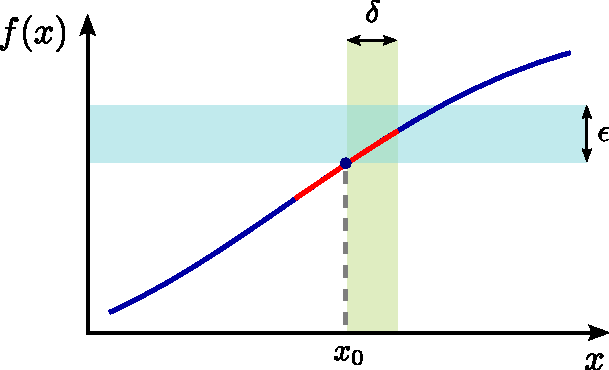
\includegraphics[width=0.5\textwidth]{continuity}
\end{figure}
    
A counter-example, with a function that has a discontinuity at some
$x_0$, is shown below. If we choose $\epsilon$ smaller than the gap,
then no matter what value of $\delta > 0$ we try, any choice of
$0 < x < \delta$ will give a value of $f(x)$ that's further than
$\epsilon$ from $f(x_0)$. Hence, the continuity condition is
violated for sufficiently small choices of $\epsilon = 1/2$, and we
say that $f$ is \textbf{discontinuous} at $x_0$.

\begin{figure}[h]
  \centering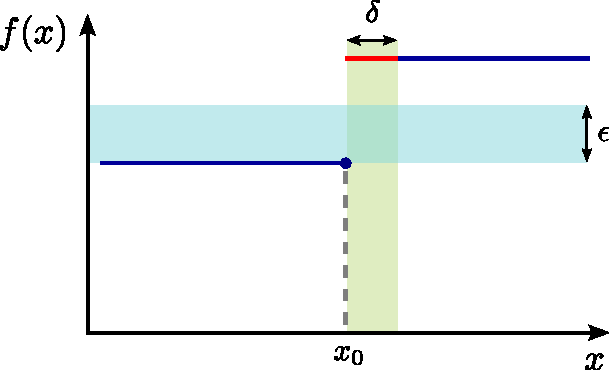
\includegraphics[width=0.5\textwidth]{discontinuity}
\end{figure}

\subsection{Exercises}
\label{exercises}

\begin{enumerate}
\item 
An alternative definition of the exponential function is the limiting
expression
\begin{equation}
  \exp(x) \equiv \lim_{n\rightarrow\infty} \left(1+\frac{x}{n}\right)^n.
\end{equation}
Prove that this is equivalent to the definition in terms of an infinite
series:
\begin{equation}
  \exp(x) \equiv 1 + \sum_{n=1}^\infty\frac{x^n}{n!}.
\end{equation}

\item
Prove that $\exp(x+y) = \exp(x)\,\exp(y)$, using the definition of the
exponential as an infinite series. Your proof must avoid using the
concept of ``raising to the power'' of a non-natural number (this is to
avoid circular logic, since this feature of the exponential function can
be used in the generalized definition of the power operation).

\item
Prove that $\exp(x) = e^x.$

\item
  A ``non-natural'' logarithm of base $c$ is defined as
  \begin{equation}
    \log_c(x) = y \quad\mathrm{where}\;\; c^y = x.
  \end{equation}
  Using the generalized definition of the power operation, derive an
  expression for the non-natural logarithm in terms of the natural
  logarithm.

\item
Prove, using trigonometry,
that
\begin{equation}
  \sin(\theta_1 + \theta_2) = \sin(\theta_1) \cos(\theta_2) + \cos(\theta_1)\sin(\theta_2).
\end{equation}
You may assume that $\theta_1, \theta_2 \in [0, \pi/2].$

\item
Prove, using the identities from Section~\ref{trigonometric-functions},
that
\begin{align}
  \cos(3x) &= 4[\cos(x)]^3 -3\cos(x) \\
  \sin(3x) &= 3\sin(x)-4[\sin(x)]^3
\end{align}
\end{enumerate}

\end{document}
